Essendo tutte le unità di misura del sito definite in \textit{em}, è possibile cambiare la dimensione del font alla base del sito per far scalare di conseguenza l'interfaccia, con buoni risultati.\\
Tuttavia, sono stati necessari alcuni accorgimenti per avere un'interfaccia mobile utilizzabile, il più radicale dei quali è stato inserire una navbar a scomparsa. Il risultato è visibile in \autoref{Fig:layoutMobile}. Ciò è stato ottenuto mediante l'inserimento di una burger icon nell'header: un tap su tale icona apre la navbar, che si sovrappone al resto della pagina. Il menù si può quindi chiudere attraverso la x posta in alto a destra.\\

\begin{figure}
	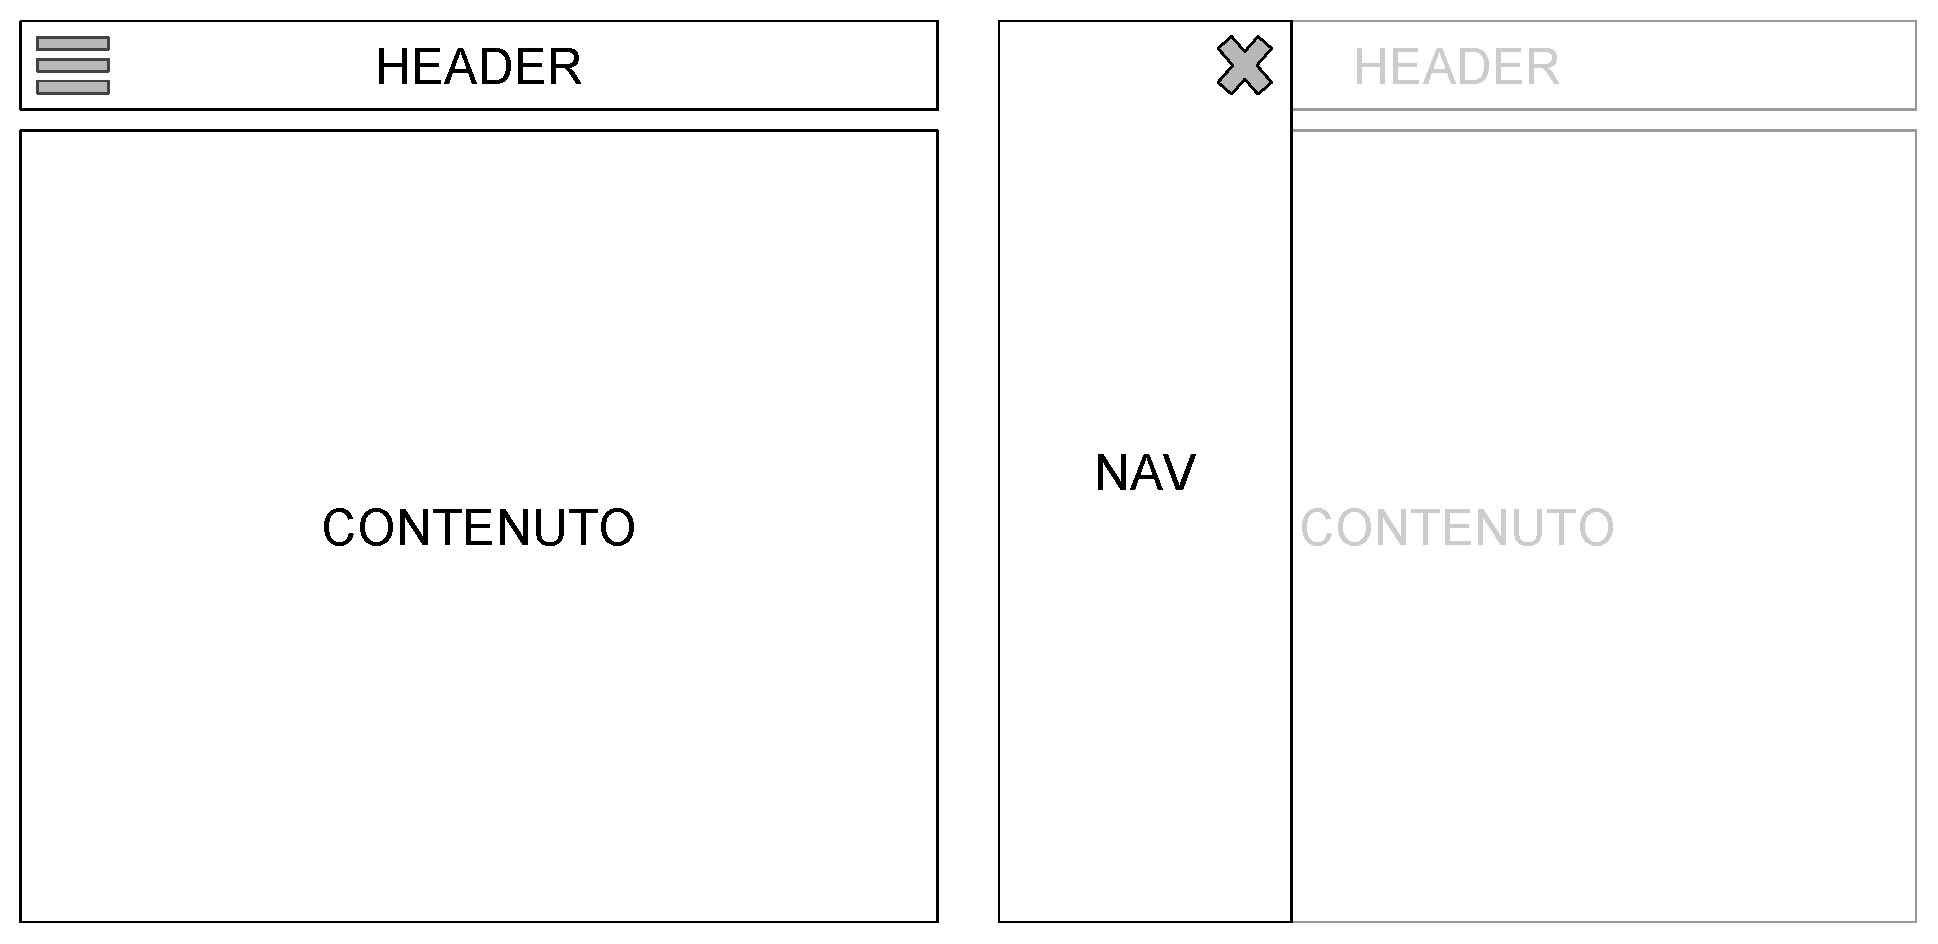
\includegraphics[width=1\linewidth]{sez/Progettazione/Layout/layout-mobile.pdf}
	\caption{Layout di una generica pagina del sito in versione mobile, a sinistra con navbar nascosta, a destra con navbar aperta}
	\label{Fig:layoutMobile}
\end{figure}

Altro dettaglio che cambia a seconda della dimensione della finestra è la visualizzazione dei risultati di ricerca di un libro, come rappresentato in \autoref{Fig:searchItems}. I risultati della ricerca vengono mostrati cercando di avere un buon compresso fra leggibilità e necessità di scrolling.

\begin{figure}
	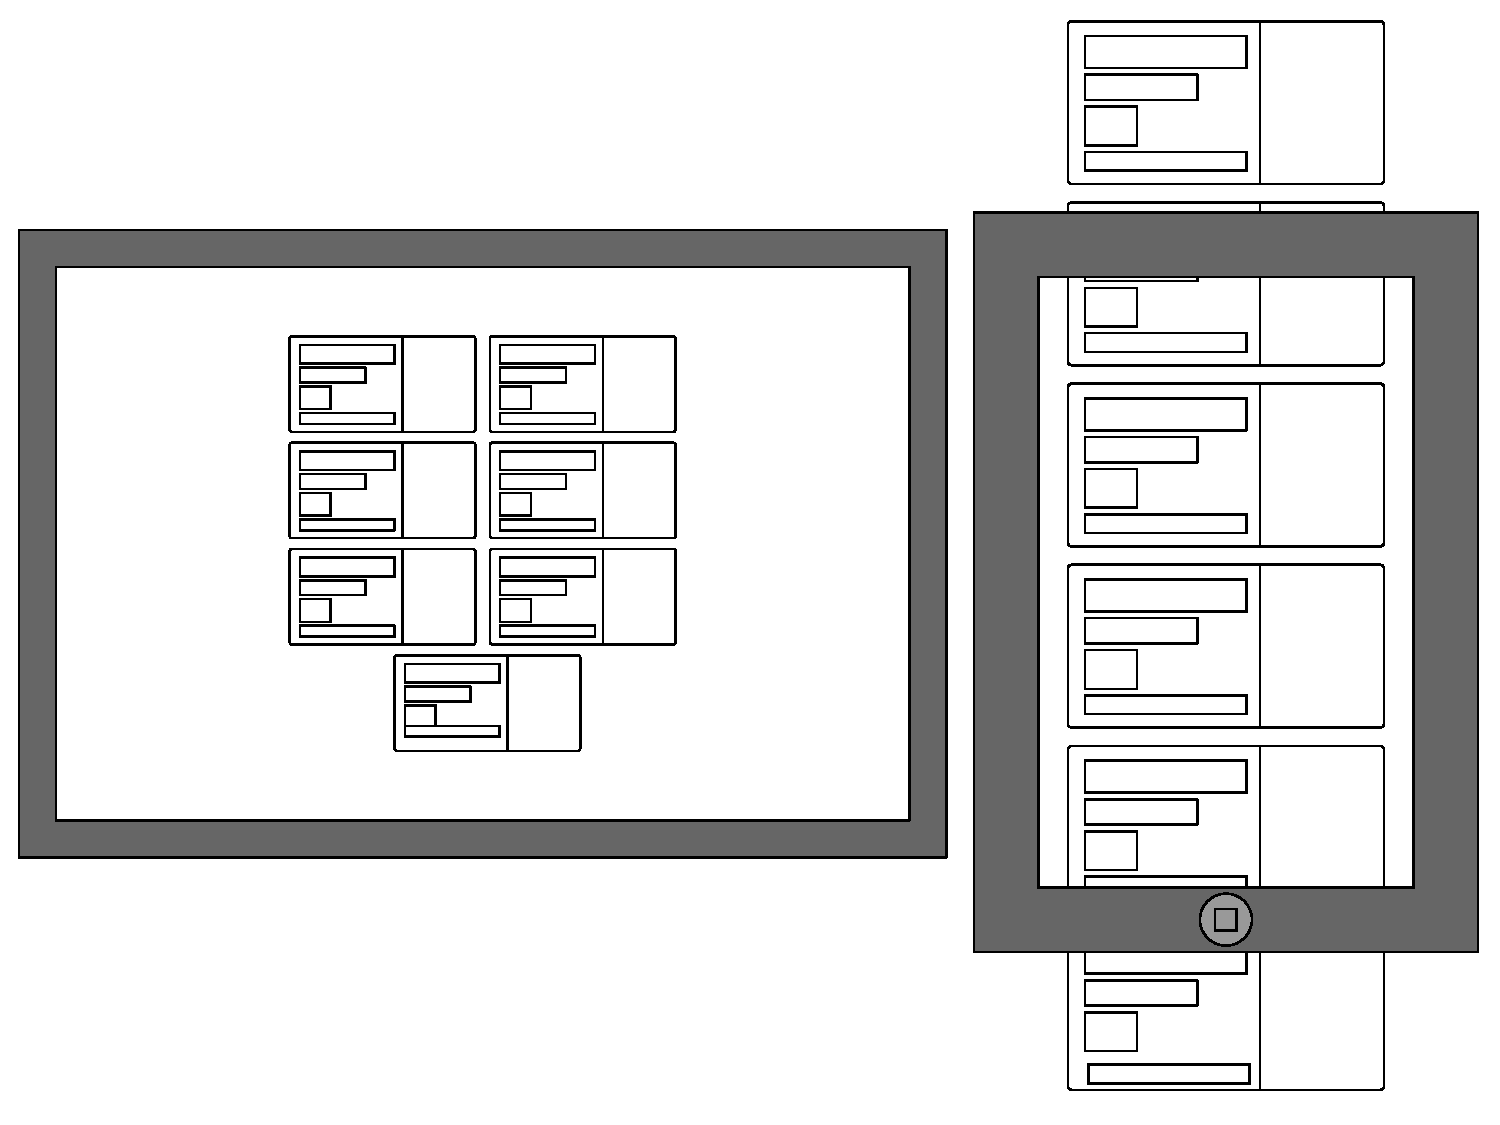
\includegraphics[width=1\linewidth]{sez/Progettazione/Layout/Search-items.pdf}
	\caption{Layout dei risultati di ricerca desktop (sinistra) e mobile (destra)}
	\label{Fig:searchItems}
\end{figure}